%%% template.tex
%%%
%%% This LaTeX source document can be used as the basis for your technical
%%% paper or abstract.

%%% The parameter to the ``documentclass'' command is very important.
%%% - use ``review'' for content submitted for review.
%%% - use ``preprint'' for accepted content you are making available.
%%% - use ``tog'' for technical papers accepted to the TOG journal and
%%%   for presentation at the SIGGRAPH or SIGGRAPH Asia conference.
%%% - use ``conference'' for final content accepted to a sponsored event
%%%   (hint: If you don't know, you should use ``conference.'')

\documentclass[tog]{acmsiggraph}
\usepackage[T1]{fontenc}
\usepackage[utf8]{inputenc}
\usepackage[swedish, english]{babel}
\usepackage{booktabs}
\usepackage{float}

%%% Make the ``BibTeX'' word pretty...

\def\BibTeX{{\rm B\kern-.05em{\sc i\kern-.025em b}\kern-.08em
    T\kern-.1667em\lower.7ex\hbox{E}\kern-.125emX}}

%%% Used by the ``review'' variation; the online ID will be printed on 
%%% every page of the content.

\TOGonlineid{45678}

%%% Used by the ``preprint'' variation.

\TOGvolume{0}
\TOGnumber{0}

\title{Perceived Depth Perception In A Virtual Environment Using A Head Mounted Display}

\author{Jesper Blidkvist\thanks{e-mail:Jesper.Blidkvist@live.se}\\Student, BTH}
\pdfauthor{Jesper Blidkvist}

\keywords{Virtual Reality, 3D, Depth Perception}

\begin{document}

%%% This is the ``teaser'' command, which puts an figure, centered, below 
%%% the title and author information, and above the body of the content.

 \teaser{
   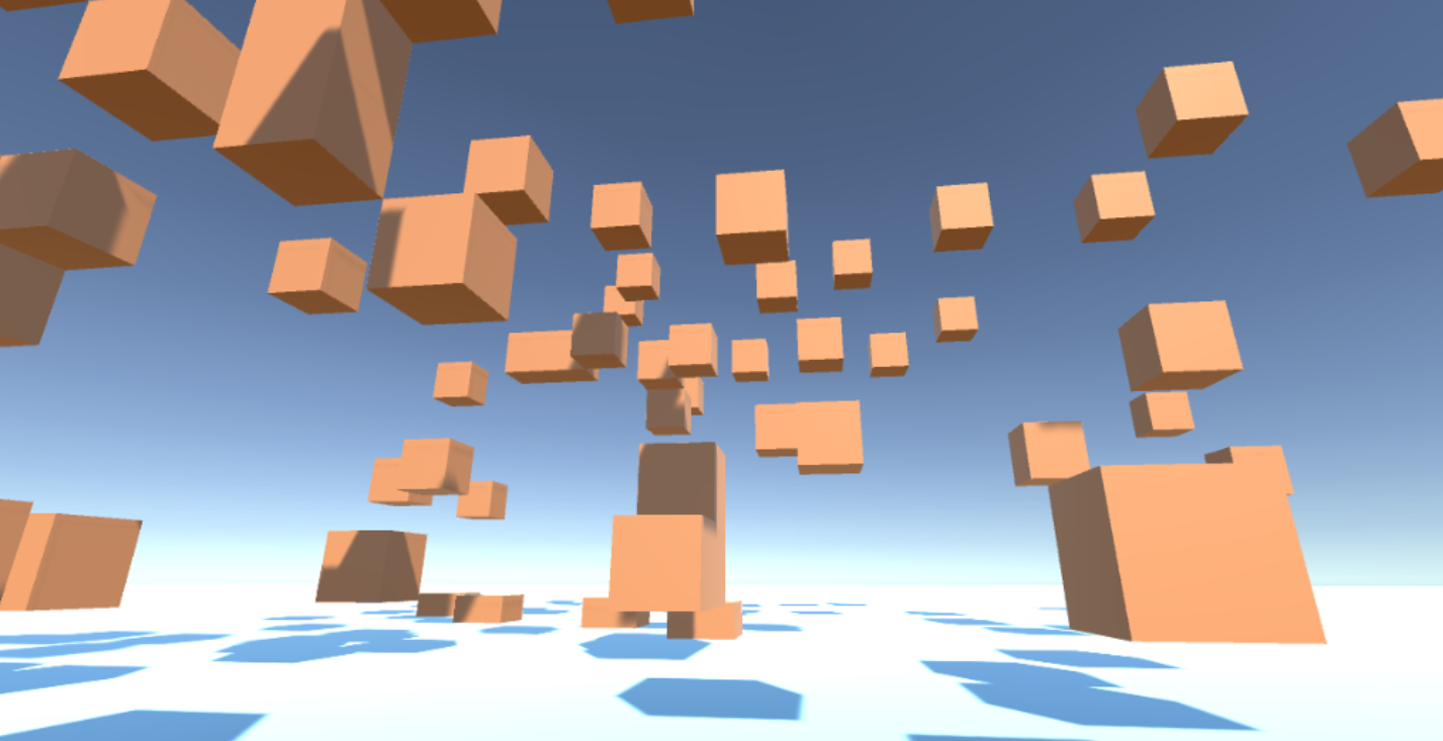
\includegraphics[height=1.5in]{images/Untitled-2}
   \caption{Environment presented to participants}
 }

\maketitle

\begin{abstract}
In order to better understand how binocular depth cues can be recreated and manipulated in a virtual environment, a small scale experiment was created in which participants where presented with a virtual scene containing a number of cubes. The subjects where asked to observe the cubes for a short while, before the distance between the virtual cameras was either increased or decreased. The participants were then asked if they noticed any differences from the previous scene. Because the test group was small, it is hard to draw any definite conclusion, but it does however seem as if there are indications that most people will notice that something change, they will however be unable to pinpoint exactly what that change is.  



\end{abstract}

\begin{CRcatlist}
  \CRcat{I.3.3}{Computer Graphics}{Three-Dimensional Graphics and Realism}{Virtual Reality}
  \CRcat{H.5.1}{Information Interfaces and Presentation}{Artificial, augmented, and virtual realities};
\end{CRcatlist}

\keywordlist


\copyrightspace

\section{INTRODUCTION}

The purpose of this paper is to investigate how humans perceive depth in a virtual 3D environment, more specifically how the distance between the two virtual cameras can influence the users perception of depth. On a pragmatic level, this could be applied in games or other virtual reality mediums to help alleviate the scale issues experienced by some users. The ability to manipulate the users perception without changing the actual geometry of a scene could also be used for example in a multiplayer horror game, where manipulation of the distance between the cameras could be used to cause various players to perceive the scene in different ways without having to change the actual geometry and the experience of the other players.

It is fairly safe to say that everyone in modern society has in some way experienced something in which depth cues are manipulated to enhance or change a persons perception of depth. From a painted picture that uses paint to create colour and shading to modern 3D movies in which among other techniques polarised lenses are used to only allow one image to on eye, and another to the other eye. The subject of recreating and manipulating depth can therefore be said to be a very broad subject perhaps now even more relevant as the continued evolution and popularity of head mounted virtual reality displays such as the Occulus rift or the Htc Vive. Because of this there has been an increase in the amount of research conducted in regards to human depth perception, and it would seem that this is a trend that is not going to change any time soon.  


\section{BACKGROUND}
In order for an observer to perceive an object and ascertain its position relative to the observers own, the brain needs to process and interpret multiple sources of information which are commonly referred to as depth cues. ~\cite {Reichelt et al:2010:DPHV}. These are often divided into two subcategories, binocular and monocular cues. In some scientific literature the term visual depth cues or pictorial depth cues is used instead of monocular cues. For the purposes of this short paper however the terms used will be binocular and monocular cues. As the names suggest, the binocular cues require the use of both eyes while the monocular cues only require one eye ~\cite {Pfautz:2002:DPCG}.

The binocular cues are a result of the brain taking advantage of the fact that each eye is placed approximately 15 cm apart horizontally on an average human adults head~\cite {Akai:1998:DPIRVR}. Because of this the retina of each eye receives a slightly different image compared to the other as result of the two different viewing angles. These two images are then merged in the striate cortex of the brain, and the difference is interpreted and used as a cue to ascertain depth ~\cite{Reichelt et al:2010:DPHV} 

\begin{figure}[ht]
	\centering
	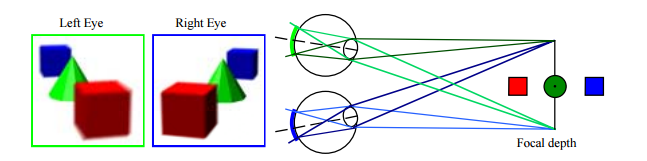
\includegraphics[width=3.0in]{images/depthCuesBinocular}
	\caption{Stereopsis. Image courtesy of David Pfaust  }
	\label{fig:DepthPerception}
\end{figure}

From this it follows that an object placed at different distances from the observer will have different amounts of binocular disparity ~\cite {Boyd:2000:DPC}. I.e, the further away an object is the more similar the two images will become. 

An easy way to test and prove this for yourself is to put your index finger along the bridge of your nose and then observe how it appears to move left and right when you close one eye and look at it with the other. Contrast this with observing the apparent movement of the finger at arms length using the same method of closing one eye and observing with the other.   
 
From this it also becomes apparent that as the distance to a given object from the observer increases, the binocular cues will become more and more useless as the images revived by each eye become more and more similar. It is said that for binocular cues to work best the distance from an observer to an object should be fairly small, approximately 30 meters or less. ~\cite {Palvqvist:2013:DPDS}.

To perceive depth at distances greater than the above mentioned thirty meters most people use monocular cues as their primary sources of depth information ~\cite {Palvqvist:2013:DPDS}. 

The monocular cues consists of perceived differences in shadows and light on an object ~\cite {Pfautz:2002:DPCG}.Things that you would normally find in a painting done by an artist, or in a video game rendered on a computer screen.

\begin{figure}[ht]
	\centering
	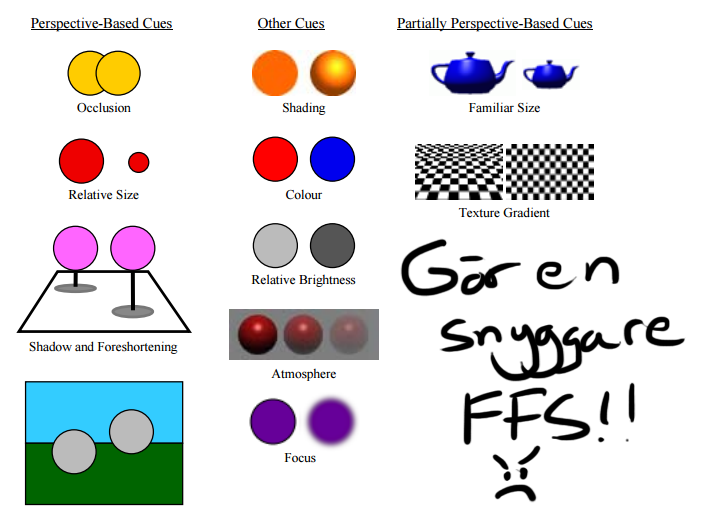
\includegraphics[width=3.0in]{images/depthCues}
	\caption{Examples of monocular depth cues. Image courtesy of David Pfaust}
	\label{fig:DepthPerception}
\end{figure}

These are for example one object occluding another object. The object occluding must logically be closer to the observer. If two objects are relative size of similar objects at different distances. The loss of detail with increased distance and motion parallax ~\cite {Pfautz:2002:DPCG}  ~\cite {Kemeny:2003:DPDSE}. These depth cues are readily found in most entertainment media, from pictures to movies. A more subtle monocular depth cue that might not be as apparent is the amount of accommodation the lens in the eye has to provide to keep an object in focus ~\cite{Pfautz:2002:DPCG}. 


It should be noted that one cue does not exclude another and as such a person observing an object at a distance within 30 meters will most likely use a combination of depth cues ~\cite {Boyd:2000:DPC}  ~\cite {Pfautz:2002:DPCG}. While the cues themselves can be said to be fairly well understood, the way in which they cooperate is somewhat disputed ~\cite {Boyd:2000:DPC} 

\section{EXPERIMENT SETUP}

The experiment was created using the Unity Game Engine developed by Unity Technologies and the Oculus Rift head mounted display by Occulus, hereafter referred to as HMD. A small amount of C\# code was also written to allow the distance between the virtual cameras to be either increased or decreased. The reason that Unity was chosen is that it would allow for a quick experiment set up without the creation of en entirely new engine, and since the latest version has native support for the Oculus HMD the interaction between the software running the experiment and the HMD would not pose a problem.
At the time of writing there are a number of HMDs available for developer, the Oculus was chosen primarily for the previously stated native support in Unity and because that was the only HMD that was easily available for the experimenter at the time of the experiment.

The scene created in unity consists of a blue skybox, a grey plane that stretches to infinity in all directions and which acts as ground and seventy five cubes of the same size and rotation that get generated upon start-up. The cubes are randomly distributed within a spaced defined as between 10 and 30 in game units away from the player in their forward facing direction, and between 0 and 25 of the in game units to the apparent left or right of the player. During start-up the program also generates a random integer. This integer will decide, depending on if it is even or odd, if the distance between the cameras will be increased or decreased during the rest of the experiment. The program writes this integer to a file so as to enable the experimenter to compare the notes taken of the participants experience with what actually changed during the experiment at a later time. This was done so that the experimenter would be unable to know whether the distance between the cameras had increased or decreased during the experiment and such would not be able to influence the participants when asking the questions. 

During the actual experiment the user is seated on a chair and puts on the HMD and adjusts it until it is placed comfortably on their head. They are then asked to look at the cubes for about thirty seconds.
The experimenter then presses a button on the keyboard which disables the rendering of the scene. The disabling of the rendering during the camera translation was done both to alleviate possible sources of nausea, but also so that the distance between the cameras could change without the participant noticing. 

Depending on if the integer generated at start-up is even or odd, the distance between the cameras is then increased and the cubes are then rendered again. Once again the participant is presented with the same scene but now with a different distance between the cameras. The participant is allowed to observe for approximately 30 seconds before the experimenter then asks a few questions:
\begin{itemize}  
	
	\item "Do you see the cubes?"
	
	\item "Is anything different, and if so what?"
	 
	
\end{itemize}

This procedure is then repeated four times with further increases or decreases.

It should be noted that a bug was discovered at the same day as the experiment was being performed. After the distance between the cameras had been increased or decreased the rig used by Unity to keep track of the two virtual cameras started to behave erratically if the participant were to start moving around in the 3D space or if they were to move their head excessively. 
This effect was at first barely noticeable but as the distance between the cameras increased or decreased the effect became exponentially worse. 

However as the participants where never meant to move around in the scene and at the start where asked to look forward and keep their head still as they could, it was believed that this bug would not influenced the results of this experiment.

\section{RESULT}

The results can be found below in table 1. Since the participants that did notice a change also noticed it for every following increase or decrease, and that the same could be said for the participants that did not notice any change, this part of the results have been abbreviated into a "yes" or "now" in the last column instead of specifying for each segment of the experiment.    

\begin{table}[H]
	\centering
	\caption{Experiment Results}
	\label{The results}
	\begin{tabular}{@{}ccccccc@{}}
		\toprule
		& Sex                         & Age                     & Vision                       & Vr Exp.                   & Inc/Dec                  & Change                   \\ \midrule
		\multicolumn{1}{|c|}{1}  & \multicolumn{1}{c|}{male}   & \multicolumn{1}{c|}{21} & \multicolumn{1}{c|}{glasses} & \multicolumn{1}{c|}{none} & \multicolumn{1}{c|}{inc} & \multicolumn{1}{c|}{Yes} \\ \midrule
		\multicolumn{1}{|c|}{2}  & \multicolumn{1}{c|}{male}   & \multicolumn{1}{c|}{20} & \multicolumn{1}{c|}{glasses} & \multicolumn{1}{c|}{none} & \multicolumn{1}{c|}{inc} & \multicolumn{1}{c|}{Yes} \\ \midrule
		\multicolumn{1}{|c|}{3}  & \multicolumn{1}{c|}{female} & \multicolumn{1}{c|}{23} & \multicolumn{1}{c|}{glasses} & \multicolumn{1}{c|}{none} & \multicolumn{1}{c|}{dec} & \multicolumn{1}{c|}{Yes} \\ \midrule
		\multicolumn{1}{|c|}{4}  & \multicolumn{1}{c|}{male}   & \multicolumn{1}{c|}{22} & \multicolumn{1}{c|}{20/20}   & \multicolumn{1}{c|}{none} & \multicolumn{1}{c|}{inc} & \multicolumn{1}{c|}{Yes} \\ \midrule
		\multicolumn{1}{|c|}{5}  & \multicolumn{1}{c|}{male}   & \multicolumn{1}{c|}{21} & \multicolumn{1}{c|}{glasses} & \multicolumn{1}{c|}{none} & \multicolumn{1}{c|}{dec} & \multicolumn{1}{c|}{Yes} \\ \midrule
		\multicolumn{1}{|c|}{6}  & \multicolumn{1}{c|}{male}   & \multicolumn{1}{c|}{21} & \multicolumn{1}{c|}{20/20}   & \multicolumn{1}{c|}{none} & \multicolumn{1}{c|}{dec} & \multicolumn{1}{c|}{Yes} \\ \midrule
		\multicolumn{1}{|c|}{7}  & \multicolumn{1}{c|}{male}   & \multicolumn{1}{c|}{20} & \multicolumn{1}{c|}{glasses} & \multicolumn{1}{c|}{none} & \multicolumn{1}{c|}{inc} & \multicolumn{1}{c|}{Yes} \\ \midrule
		\multicolumn{1}{|c|}{8}  & \multicolumn{1}{c|}{male}   & \multicolumn{1}{c|}{28} & \multicolumn{1}{c|}{20/20}   & \multicolumn{1}{c|}{none} & \multicolumn{1}{c|}{dec} & \multicolumn{1}{c|}{Yes} \\ \midrule
		\multicolumn{1}{|c|}{9}  & \multicolumn{1}{c|}{male}   & \multicolumn{1}{c|}{20} & \multicolumn{1}{c|}{lenses}  & \multicolumn{1}{c|}{none} & \multicolumn{1}{c|}{inc} & \multicolumn{1}{c|}{No}  \\ \midrule
		\multicolumn{1}{|c|}{10} & \multicolumn{1}{c|}{male}   & \multicolumn{1}{c|}{24} & \multicolumn{1}{c|}{glasses} & \multicolumn{1}{c|}{none} & \multicolumn{1}{c|}{inc} & \multicolumn{1}{c|}{Yes} \\ \midrule
		\multicolumn{1}{|c|}{11} & \multicolumn{1}{c|}{male}   & \multicolumn{1}{c|}{22} & \multicolumn{1}{c|}{20/20}   & \multicolumn{1}{c|}{none} & \multicolumn{1}{c|}{inc} & \multicolumn{1}{c|}{No}  \\ \bottomrule
	\end{tabular}
\end{table}

	
		The replies given when asked to describe what had changes these are the responses can be found in table 2 below. It should be noted that the replies are group together under four main underlying statements identified during the experiment. It should also be noted that participant 9 and 11 are not included in this table as they did not notice any change what so ever.
		
	\begin{table}[H]
		\centering
		\caption{Statements sorted by frequency}
		\label{Answers}
		\begin{tabular}{@{}ll@{}}
		\toprule
		Statment                  & Uttered by:      \\ \midrule
		"do not know"             & 1, 3, 6, 7, 8,10 \\
		"the cubes moved"         & 2, 4             \\
		"the depth had decreased" & 5                \\ \bottomrule
	\end{tabular}
\end{table}
		
		
	

\section{DISCUSSION}
It is easy to note that the group of participants is very homogeneous, the majority of the participants being males in their early twenties  with glasses which makes it difficult to make any conclusive statements about how people in general would react to the experiment. Another side effect of the small participant group that immediately becomes apparent is that the random distribution of who got increasing distance between the cameras versus the people who got decreasing distance slightly uneven, making it harder still to make any statements about the effect of decreasing the camera distance. Had there been more participants this would obviously have resolved itself as any disparity would have eventually evened itself out. 

As can be seen everyone except participant 9 and 11 noticed that something had changed. It was however difficult for the participants to pinpoint exactly what this was. There could be a number of reason why that is but one apparent is that the effect achieved by moving the cameras is not one that most people would experience in real life. Baring some sort of hideous accident a persons eyes will generally remain in their fixed location. As this change is something that most people have never experienced it would of course be hard to tell that this is what had happened. 

Another thing to consider is the participants lack of any previous experience in Virtual Reality. There is the possibility that it might be that the experience of being placed in a virtual environment where you are able to look around and observe objects in 3D in itself served as a possible distraction detracted from the task at hand. After all, at the time of writing, as is apparent from the fact that all participant answered no to the question if they had any previous experience in virtual reality, this is currently not widespread technology. 

 Another possibility is that the featureless cubes where a bad choice of objects to uses as reference points for the participants. After all, even though all the cubes are 1x1x1 in game units, equivalent to 1x1x1 meters, there is really not i would assume, a real world equivalent to that for most people. Without a frame of reference the apparent size of an object would become somewhat useless. Perhaps an object like a chair, a table, or even a simple model of a human being would have made it easier to detect if something changed and what it was that changed. 
 
 It can also be noted that the majority of participants did not have perfect vision. This might have posed a problem had the person in question had a large disparity in their vision in one eye compared to the other, but as it was all participants had more or less the same near-sightedness or far-sightedness in both eyes. And as everyone was wearing either glasses or lenses this should however not have any effect on the results. 
 
\section{CONCLUSIONS}
Due to the small group of participants it is hard to draw any general conclusions. What can however be said is that while most people did notice that something had changed most where unable to pinpoint exactly what it was that had changed. The one exception from this was participant number 5 who upon the last decrease of the distance between the cameras commented that the scene now lacked the sense of depth that it had at the beginning of the experiment.



\section{FUTURE WORK}

One of the most obvious things to think about if redoing or building upon this experiment would be to improve on the code. As stated, the code used caused some issues with the rig used by unity to render the two cameras and while it was still possible to move, it did cause some artefacts and as such the participants where asked to keep their head still and face forward.

It would also be interesting to instead of the cubes fill the scene with objects more familiar to the participants from real life. For example instead of the cubes, an experiment might be designed that uses models of cars or something similar that the participants would have more experience of what the size of a car should be in real life, thus perhaps making any distance estimations more correct 

This experiment focused on translating the cameras to increase or decrease the distance between them and thus change the angle between the two images revived by the eyes in the HMD. Another way to do this, and perhaps a better way, would be to instead rotate the virtual cameras ever so slightly to achieve a similar effect. This would also perhaps alleviate some of the issues found when translating the cameras and perhaps also achieved a change more similar to one that we experience in everyday life, after all, when we look at something close to us the eyes rotate to point at this object.

Another slightly different thing to focus on in a future experiment would be to try to remove as many other depth cues as possible and run the experiment again, or perhaps even the other way around. 

As mentioned previously there is also the fact the newness of the experience might have played a part in distracting the participants. Perhaps in the future virtual reality HMD such as the one used in the experiment will be more common and eliminate this variable. Otherwise a future experiment might consider letting the participants "train" in VR for a while beforehand playing a game or something similar to make the experiment situation feel more normal.

\section{Contact Information}

If you have questions or suggestions regarding this document, please
contact Jesper Blidkvist at ``Jesper.Blidkvist@live.se''.


\bibliographystyle{acmsiggraph}
\nocite{*}
\bibliography{template}
\end{document}
